\documentclass[10pt, xcolor={dvipsnames}]{beamer}
\usepackage{graphicx}
\usepackage{amsmath}
\usepackage{booktabs}
\usepackage[style=authortitle,
            autocite=footnote,
            backend=biber,
           ]{biblatex}
\usepackage{multirow}
\usepackage{adjustbox}
\usepackage[font=scriptsize]{caption}
\usepackage{subcaption}
\usepackage{hyperref}
\usepackage[ruled]{algorithm2e}
\usepackage{algorithmic,float}
\usepackage{dirtytalk}
\usepackage{marginnote}
\usepackage{tikz}
\usepackage[T1]{fontenc}
\usepackage{transparent}
\usepackage{eso-pic}
\usepackage{lipsum}
\usepackage{wrapfig}
\usepackage{tabularx}
\usepackage{soul}
\usepackage{array}
\usepackage[absolute,overlay]{textpos}
  \setlength{\TPHorizModule}{1mm}
  \setlength{\TPVertModule}{1mm}
%\usepackage{MnSymbol}

\newcolumntype{M}[1]{>{\centering\arraybackslash}m{#1}}

\SetKwInOut{Parameter}{parameter}

\captionsetup[figure]{labelsep=period}
\captionsetup[subfigure]{labelformat=simple}
\renewcommand\thesubfigure{\thefigure.\alph{subfigure}.}


\setbeamertemplate{navigation symbols}{}
\setbeamertemplate{caption}[number]
\bibliography{Bibliography}

\graphicspath{{/Users/flavioforenza/Desktop/latex/images/}}

% \defbeamertemplate{footline}{left page number}
% {%
%   \hspace*{0.2cm}%
%   \usebeamercolor[fg]{page number in head/foot}%
%   \usebeamerfont{page number in head/foot}%
%   \insertpagenumber\,/\,\insertpresentationendpage%
%   \hspace*{0.2cm}\vskip2pt%
% }
% \setbeamertemplate{footline}[left page number]
\setbeamertemplate{footline}[frame number]


\usetheme{Darmstadt}


%\title[short]{UNIVERSITÀ DEGLI STUDI DI MILANO}
\title[]{Distilled-Single-Shot-Detector (DSSD): un nuovo modello di guida autonoma ad alta inferenza}

\author[Flavio Forenza]{
                        
\includegraphics[scale = 0.05]{
                                        unimilogo.png}\\ 
                                        \vspace{0.1cm}
                                        \fontfamily{cmr}\selectfont {\bfseries{UNIVERSITÀ DEGLI STUDI DI MILANO}}\\
                                        \fontfamily{cmr}\selectfont \emph{Laurea magistrale in Informatica}\\
                                        \vspace{1cm}
                                        }
\date{\scriptsize Aprile 2022}

\begin{document}

\begin{frame}
    \maketitle
    \vspace{-2.5cm}
    \begin{minipage}{\linewidth}
        \centering
        \begin{minipage}{0.45\linewidth}
            \begin{flushleft}
                \emph{Relatore:}\\
                Prof. Vincenzo Piuri\\
                \emph{Correlatore:}\\
                Dott. Angelo Genovese
            \end{flushleft}
        \end{minipage}
        \begin{minipage}{0.45\linewidth}
            \begin{flushright}
                \emph{Laureando:}\\
                Flavio Forenza
            \end{flushright}
        \end{minipage}
    \end{minipage}
\end{frame}

\logo{{\vspace{-1.5cm}\reflectbox{\hspace{-1cm}\rotatebox[origin=c]{-40}{\fontsize{20mm}{15mm}\selectfont{\transparent{0.3}
\includegraphics[width=0.2\linewidth]{unimilogo_reflect.png}}}}}}


\section{"Distilled-Single-Shot-Detector (DSSD): un nuovo modello di guida autonoma ad alta inferenza"}
%\section{\centering{"Distilled-Single-Shot-Detector (DSSD): un nuovo modello di guida autonoma ad alta inferenza"}}

\begin{frame}{STATO DELL'ARTE - OBIETTIVO}
    Ricerca basata sullo sviluppo e sull'implementazione di grandi modelli deep learning in sistemi a 
    limitate risorse computazionali (es: embedded, mobile, indossabbili, etc.).\\
    Requisiti da soddisfare:\\
    \hspace{1cm}
    \begin{minipage}{\linewidth}
        \centering
        \begin{minipage}{0.45\linewidth}
            \begin{enumerate}
                \item Buona velocità di inferenza
                \item Risparmio energetico
                \item Minor occupazione della memoria
                \item Basso impatto sull'accuratezza
                \item Miglior gestione delle risorse HW/SW
            \end{enumerate}
        \end{minipage}
        \begin{minipage}{0.45\linewidth}
            \begin{figure}
                \centering
                
\includegraphics[width = \linewidth]{objective.png}
                \centering
            \end{figure}
        \end{minipage}
    \end{minipage}
\end{frame}
\begin{frame}{CRISI DEI SEMICONDUTTORI}
    
\end{frame}
\begin{frame}{LAVORO DI TESI}
    Lo studio della tesi si è concentrato sulla ricerca e sull'implementazione 
    di varie tecniche di compressione e, allo stesso tempo, di ottimizzazione, 
    in grado di offrire supporto allo sviluppo di un nuovo modello di guida autonoma efficiente e ad alta velocità di inferenza.\\
    \vspace{0.3cm}
    Quest'ultimo, deriva dallo studio di due modelli già noti allo stato dell'arte:
    \begin{minipage}{\linewidth}
        \centering
        \begin{minipage}{0.45\linewidth}
            \begin{enumerate}
                \item {\bfseries{\emph{MobileNet-V1}}}\footnotemark[1]: specializzato nel task di \emph{Image classification};
                \item {\bfseries{\emph{Single-Shot-Detector (SSD)}}}\footnotemark[2]: specializzato nel task di \emph{Object Detection}.
            \end{enumerate}
        \end{minipage}
        \begin{minipage}{0.45\linewidth}
            \begin{figure}
                \centering
                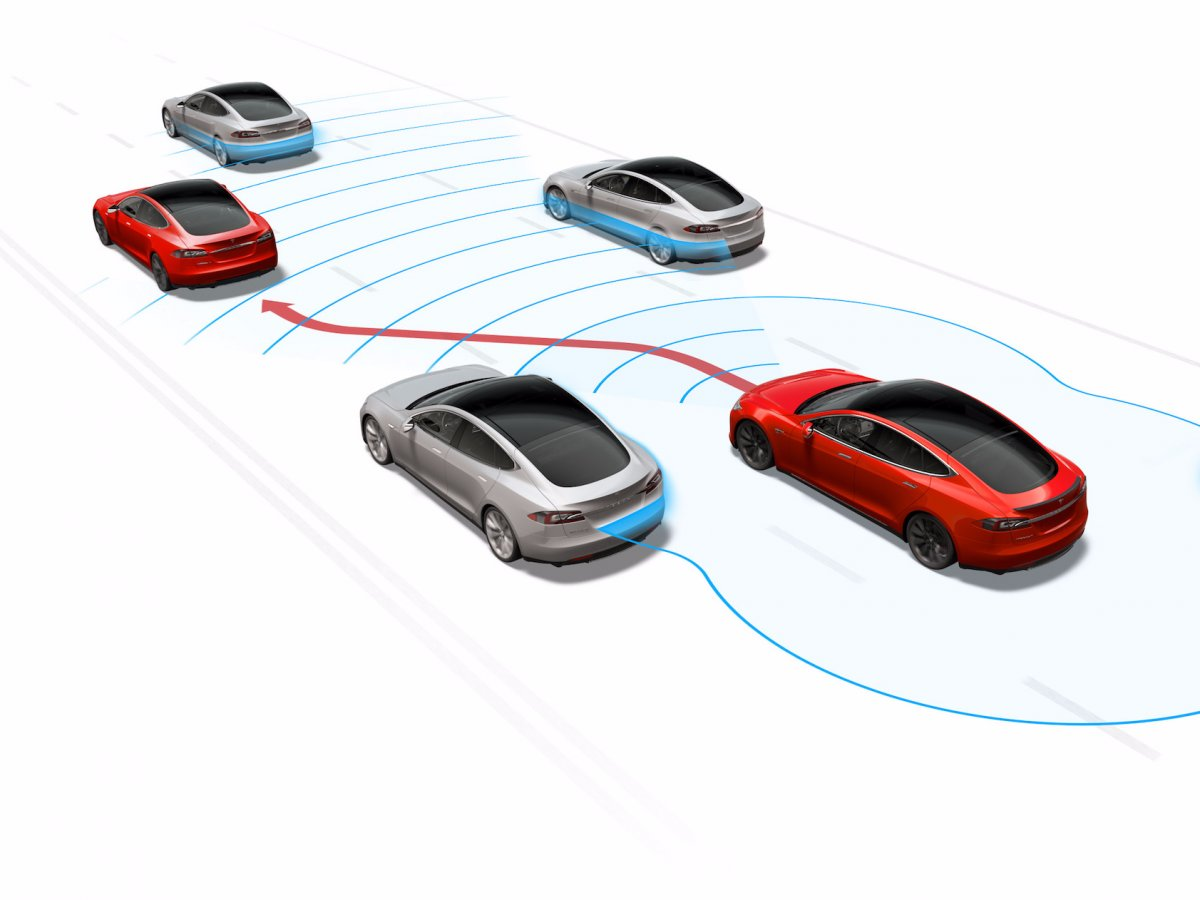
\includegraphics[width = \linewidth]{tesla_autopilot.png}
                \centering
            \end{figure}
        \end{minipage}
    \end{minipage}
    \footnotetext[1]{\emph{Andrew G. Howard et al., "MobileNets: Efficient Convolutional Neural Networks for Mobile Vision Applications", 2017.}}
    \footnotetext[2]{\emph{Liu et al., "SSD: Single Shot MultiBox Detector", 2016.}}
\end{frame}
\begin{frame}{METODOLOGIA}
    \begin{minipage}{\linewidth}
        \centering
        \begin{minipage}{0.40\linewidth}
            Per dimostrare la veridicità dei miglioramenti introdotti dal modello proposto, vengono presi come riferimento le performance ricavate dai benchmarks effettuati su diversi modelli pre-addestrati.\\
            \\
            Sia i risultati che il modello proposto, sono ottenuti tramite il flusso di esecuzione riportato nella figura accanto.
        \end{minipage}
        \hspace{0.3cm}
        \begin{minipage}{0.55\linewidth}
            \begin{figure}
                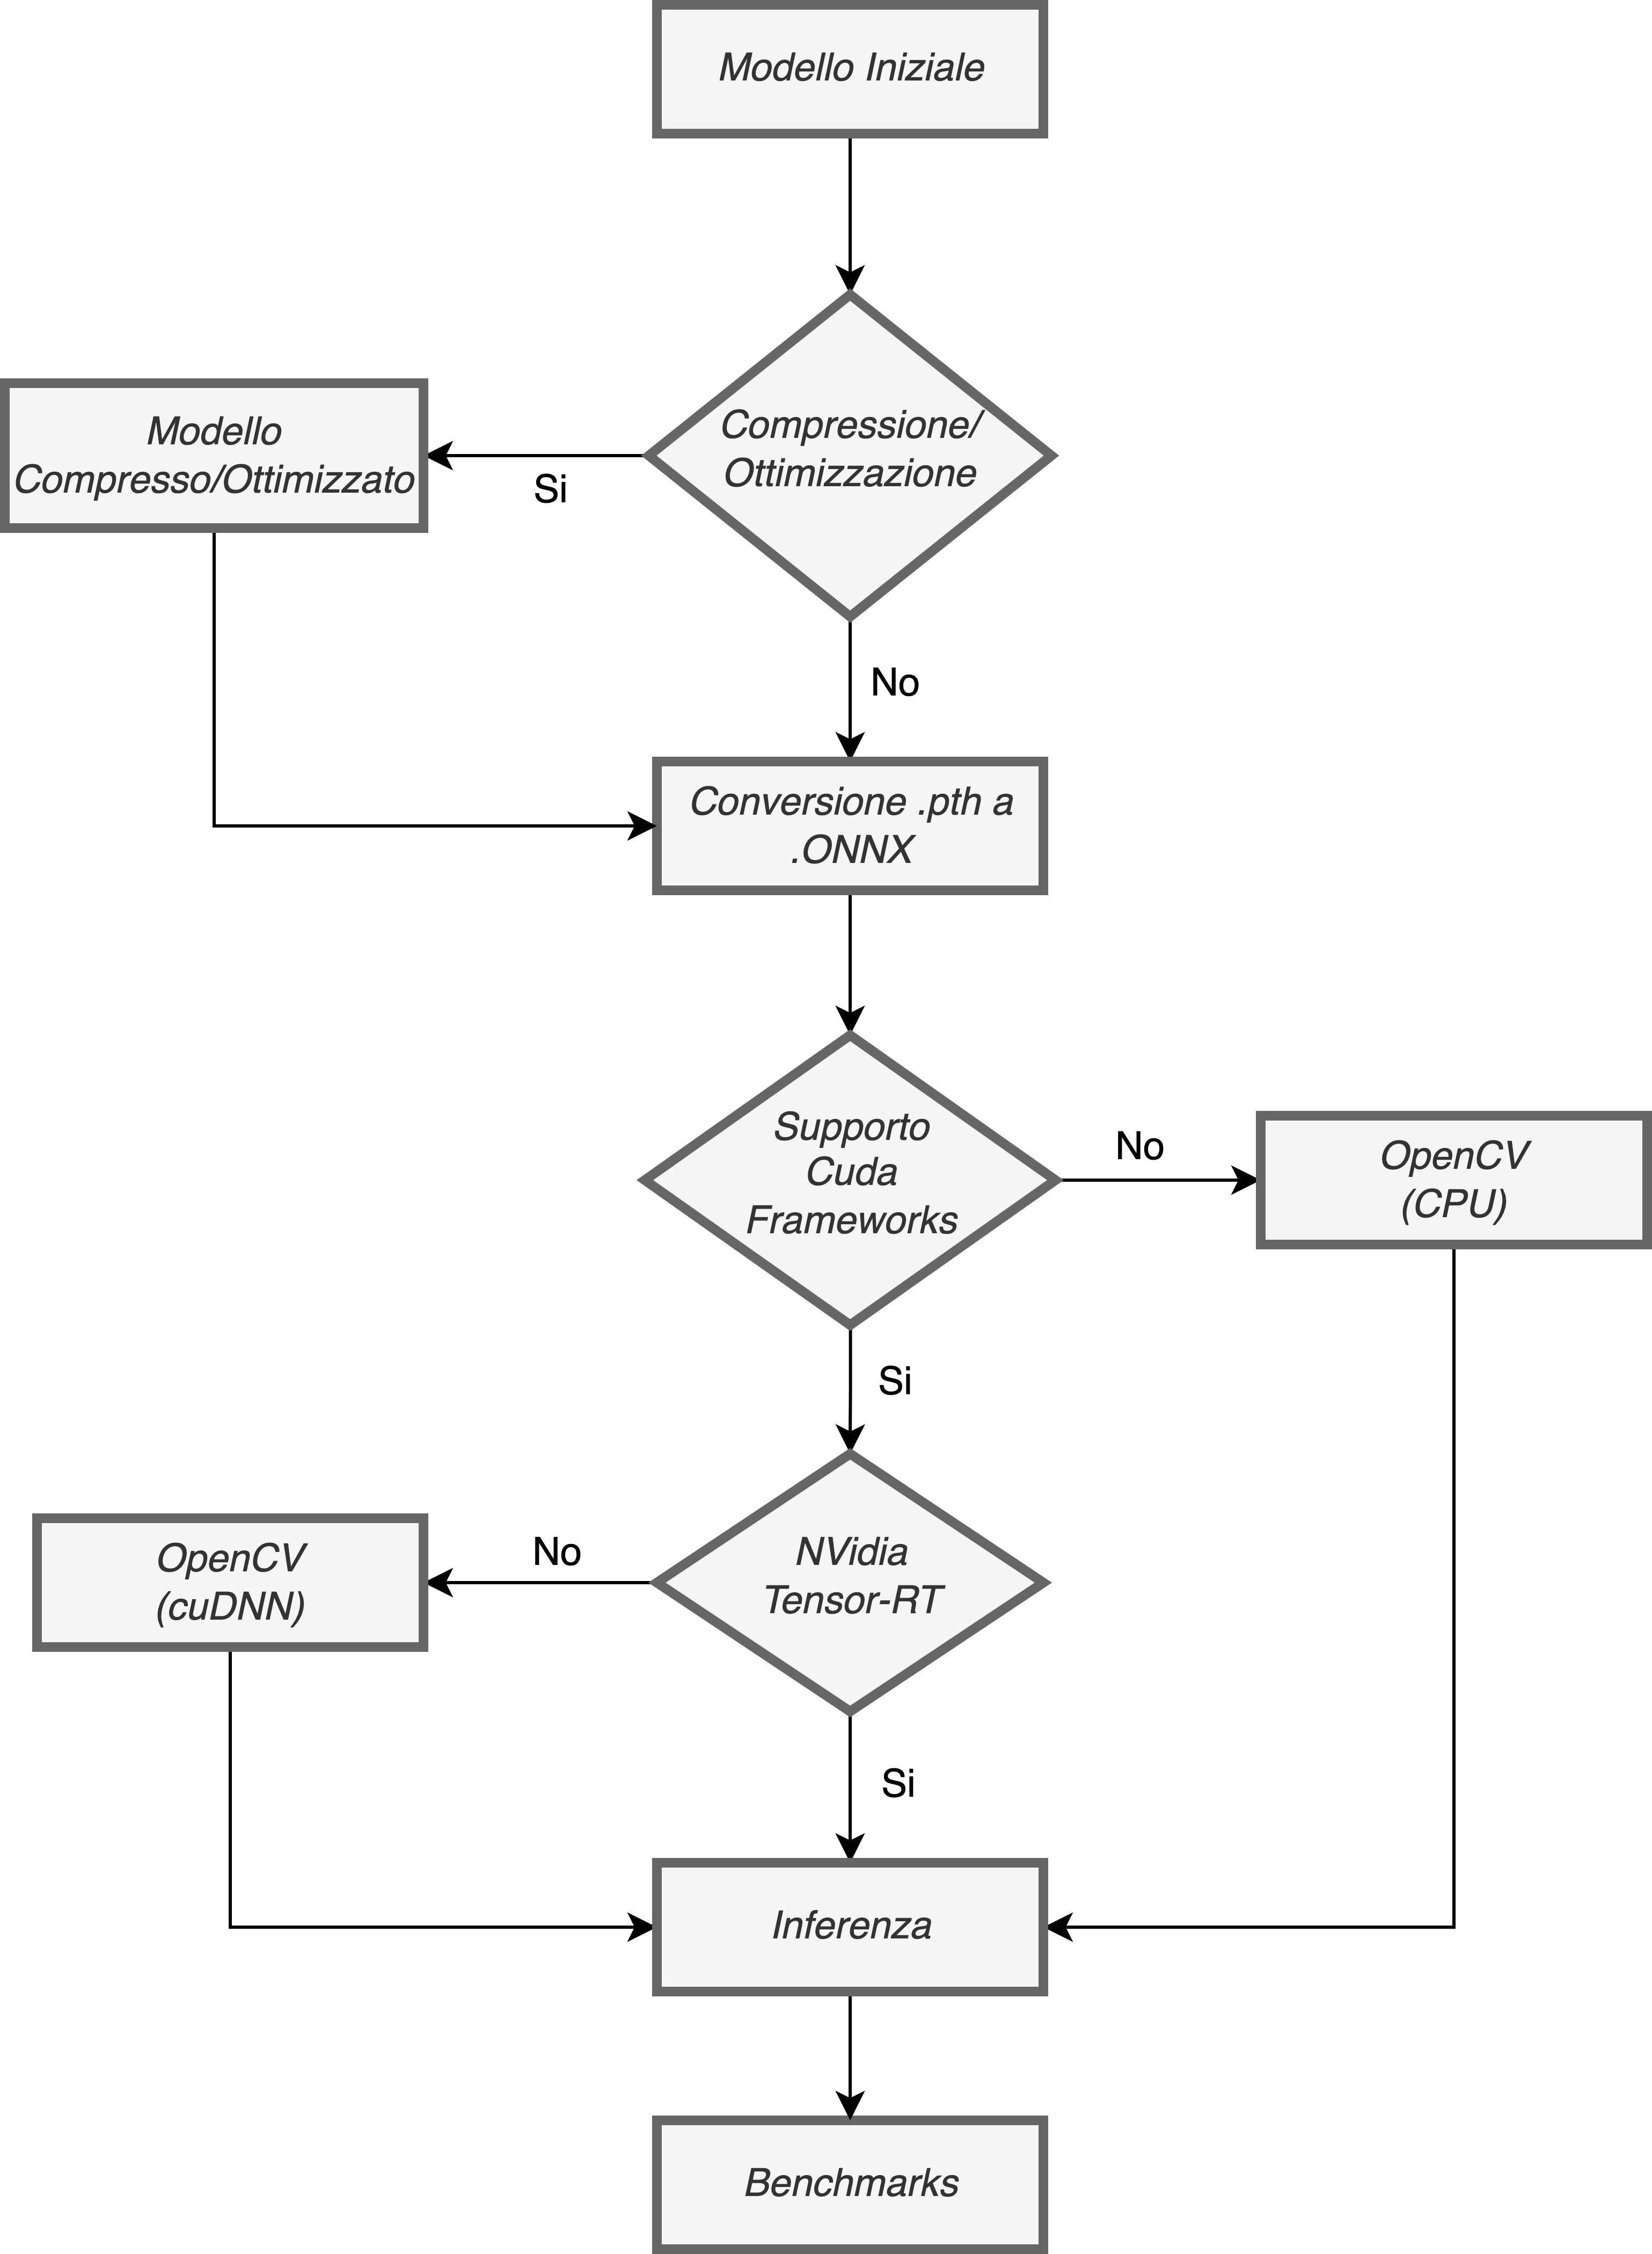
\includegraphics[width = 0.95\linewidth]{flow_chart_transparent.png}
            \end{figure}
        \end{minipage}
    \end{minipage}    
\end{frame}

\begin{frame}{ARCHITETTURE DI RIFERIMENTO}
    Tutti i test sono stati eseguiti su tre architetture differenti in termini di performance, dimensioni e costo.
     
    
\end{frame}
\begin{frame}{DATASET}
    
\end{frame}
\begin{frame}{TECNICHE DI COMPRESSIONE/OTTIMIZZAZIONE}
    Tecniche di compressione/ottimizzazione più diffuse allo stato dell'arte:
    \begin{enumerate}
        \item {\bfseries{\emph{Quantization}}}{\renewcommand{\thefootnote}{\fnsymbol{footnote}}\footnote[1]{\scriptsize \bfseries A causa dell'incompatibilità dalla Jetson Nano, la tecnica di quantizzazione non verrà approfondita. L'intero elaborato è concentrato sulle restanti due tecniche di compressione.}}: Riduzione della rappresentazione di ogni singolo bit;
        \item {\bfseries{\emph{Pruning}}}\footnotemark[3]: Azzeramento di determinati parametri nella rete;
        \item {\bfseries{\emph{Knowledge Distillation}}}\footnotemark[4]: Trasferimento della "Conoscenza" da un modello di grandi dimensioni, verso un modello più piccolo. 
    \end{enumerate}
    \footnotetext[3]{\emph{Salama A., "Pruning at a glance: Global neural pruning for model compression", 2019}}
    \footnotetext[4]{\emph{Geoffrey H. et al., "Distilling the Knowledge in a Neural Network", 2015}}
\end{frame}
\begin{frame}{PRUNING}
    \begin{figure}
        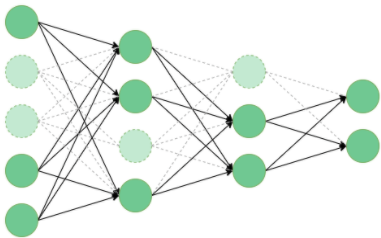
\includegraphics[width = 0.4\linewidth]{pruning no name.png}
    \end{figure}
    Mediante un indice di {\bfseries{\emph{sparsità}}}, è in grado di azzerare determinati elementi presenti nella rete.
    Il modello su cui è stata applicata tale tecnica è il \emph{Single-Shot-Detector (SSD)}.
    Esistono tre tipi di pruning:
    \begin{enumerate}
        \item {\bfseries{\emph{Structured}}}: rimuove interi filtri (canali);
        \item {\bfseries{\emph{Unstructured}}}: rimuove i parametri (es: pesi e bias) in un layer;
        \item {\bfseries{\emph{Global-Unstructured}}}: rimuove i parametri su più layer.
    \end{enumerate}
    Il framework utilizzato, avente già le API dedicate, è \emph{PyTorch}.\\
    {\textcolor{red}{\textbf{\ul{Problema}}}}: {\bfseries{Non esiste un framework in grado di eliminare le parti azzerate (TensorFlow compreso)}}.
\end{frame}
\begin{frame}{RISULTATI SPERIMENTALI - PRUNING}
    
\end{frame}
\begin{frame}{KNOWLEDGE DISTILLATION}
    \begin{figure}
        \centering
        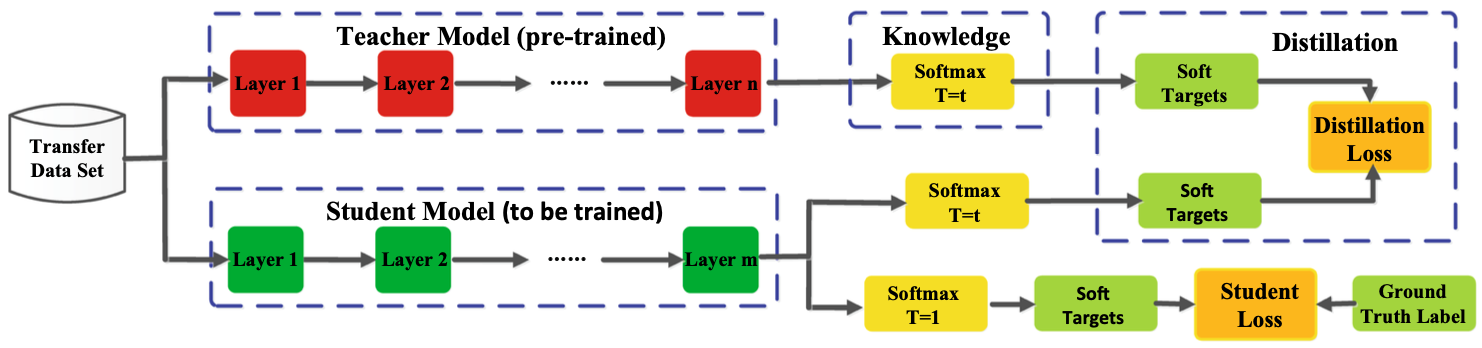
\includegraphics[width = 0.9\linewidth]{KD_losses.png}
        \centering
        \caption{Generazione cross-entropy $L_{soft}$ (in alto) e $L_{hard}$ (in basso).}
        \label{l_hard_soft}
    \end{figure}
    \vspace{-0.3cm}
     Applicata principalmente per task di \emph{image classification}, ha l'obiettivo di addestrare un modello {\bfseries{\emph{"Studente"}}} grazie all conoscenza distillata trasferita da un modello {\bfseries{\emph{"Insegnante"}}}.
     \begin{minipage}{\linewidth}
        \centering
        \begin{minipage}{0.45\linewidth}
            Elementi chiave:
            \begin{itemize}
                \item {\bfseries{\emph{Temperatura $T$}}};
                \item {\bfseries{\emph{Soft-targets}}};
                \item {\bfseries{\emph{Perdita complessiva}}}.
            \end{itemize}
        \end{minipage}
        \begin{minipage}{0.40\linewidth}
            \begin{block}{\centering Soft-targets}
                \centering
                $ q_j = \frac{e^{z_j/T}}{\sum_{k=1}^K e^{z_k/T}} $
            \end{block} 
            \begin{block}{\centering Total Loss}
                \centering \small $ L= L_{hard}+T^2L_{soft} $
            \end{block}
        \end{minipage}
    \end{minipage}
\end{frame}
\begin{frame}{METODOLOGIA PROPOSTA}
    \begin{figure}
        \centering
        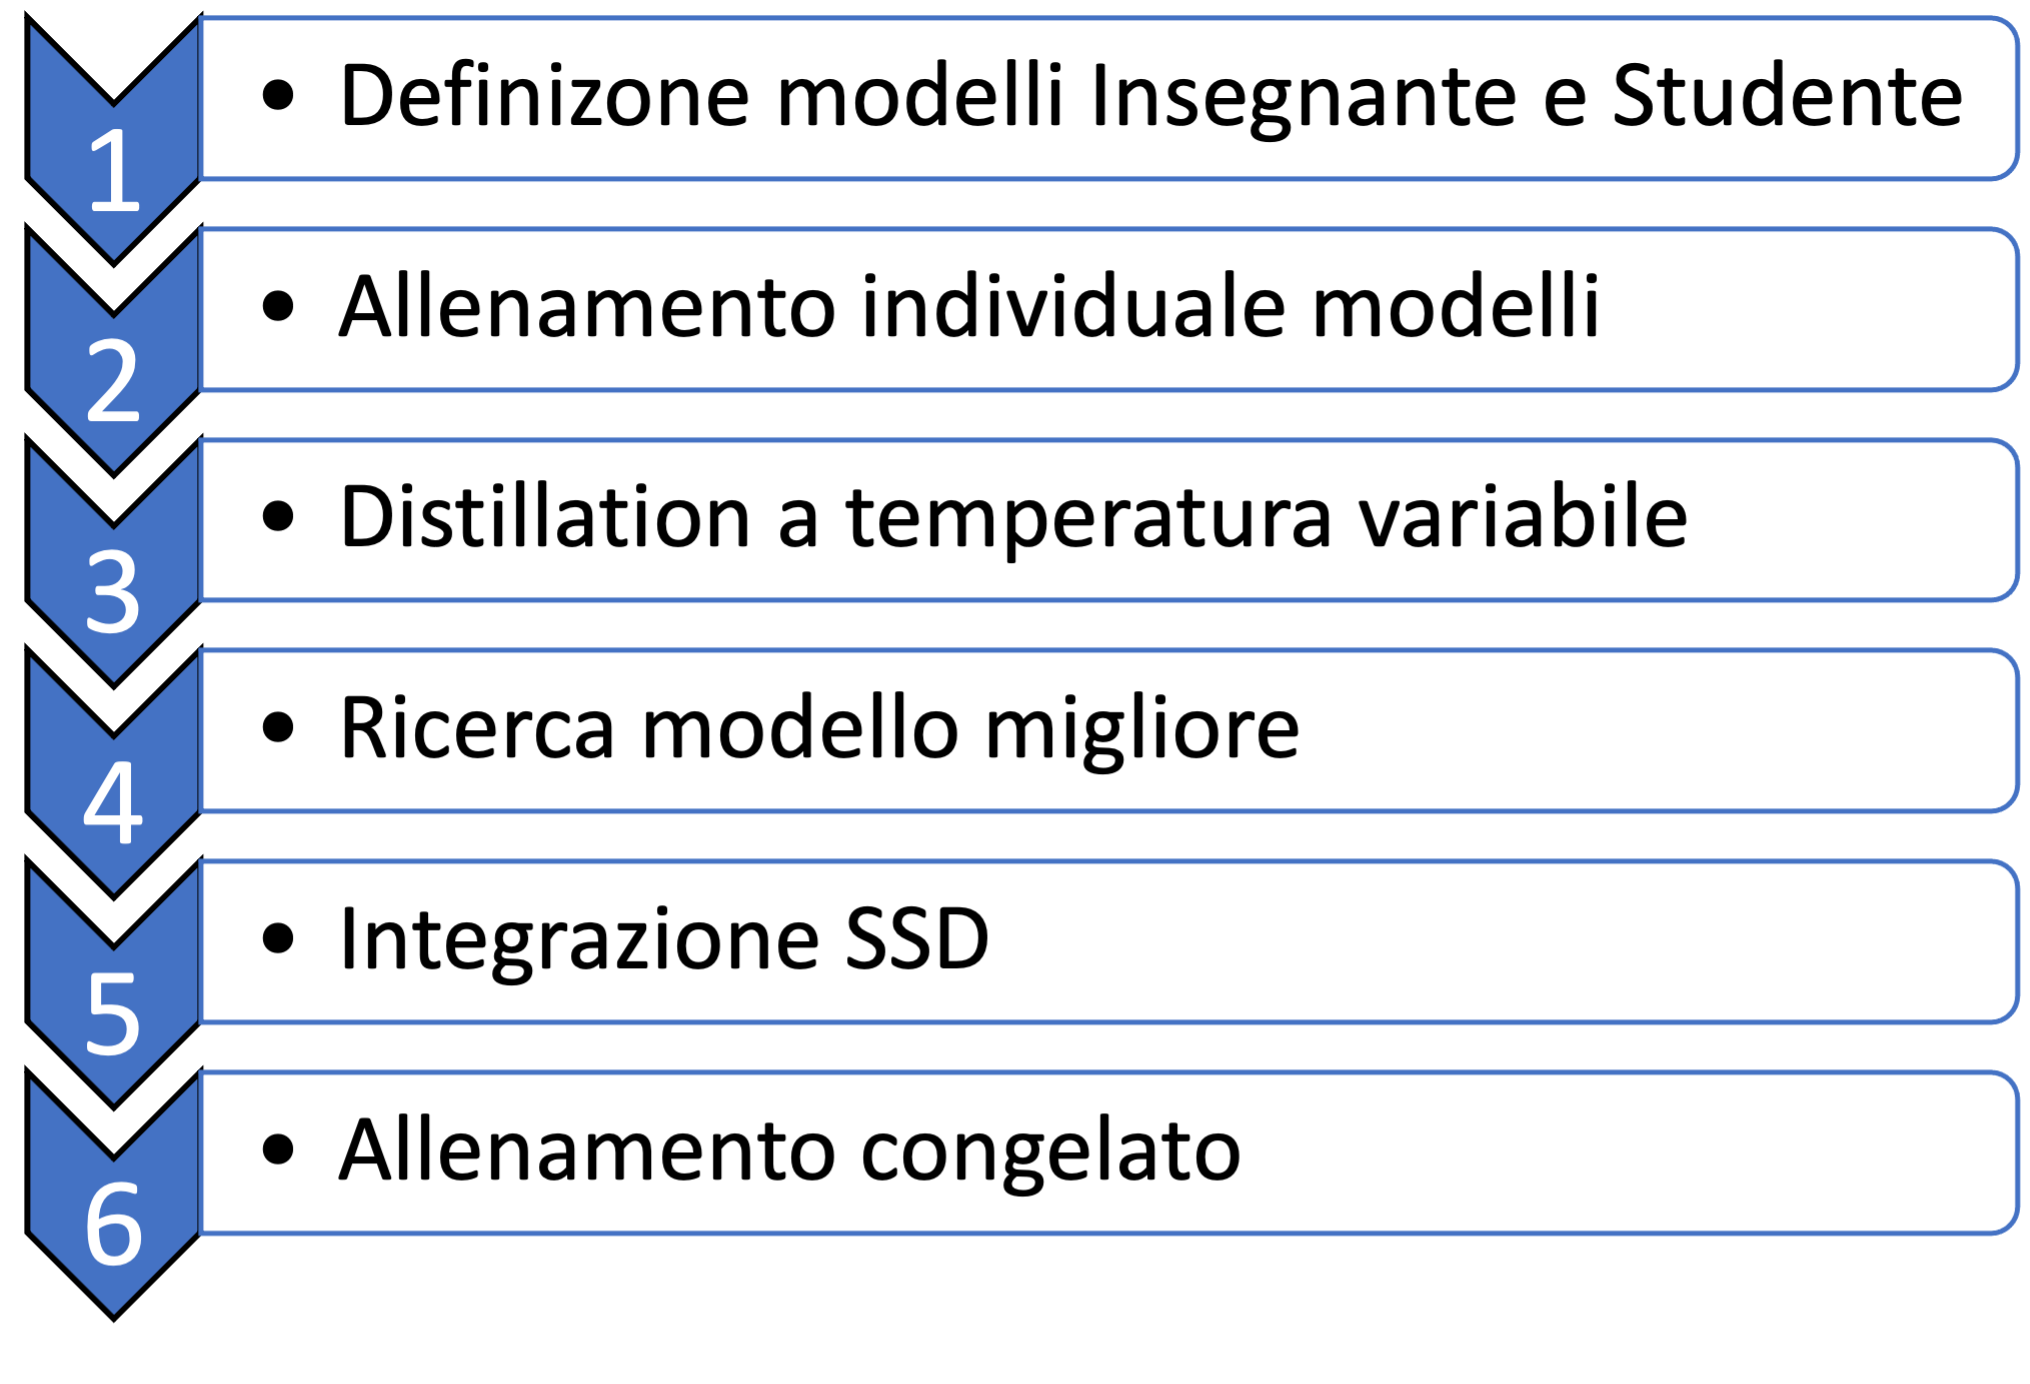
\includegraphics[width =0.7\linewidth]{steps_KD.png}
        \centering
        \caption{Steps per la creazione del modello proposto.}
    \end{figure}
    \alert{\textcolor{blue}{\textbf{{Obiettivo}}}}: utilizzare la tecnica di Knowledge Distillation per derivare un 
    modello utile per l'attività di {\bfseries{\emph{\ul{Object Detection}}}} nella guida autonoma.
\end{frame}



\begin{frame}{MODELLI INSEGNANTE E STUDENTI}
  {\bfseries{\scriptsize{(Steps 1, 2, 3 e 4)}}}
  \renewcommand{\thefootnote}{\fnsymbol{footnote}}
  \begin{minipage}{\linewidth}
    \centering
    \begin{minipage}{0.45\linewidth}
      \begin{enumerate}
        \item {\bfseries{\emph{Modelli}}}: tutti basati sulla rete {\bfseries{\emph{MobileNet-V1}}} con iper-parametro $\alpha$\footnotemark[1] variabile;
        \item {\bfseries{\emph{Allenamento}}}: individuale su un totale di 1000 epoche;
        \item {\bfseries{\emph{Distillation}}}: generazione dei modelli \emph{Studenti Distillati (Dst)} a temperatura $T$ variabile;
        \item {\bfseries{\emph{Selezione}}}: per $T>1$, il modello con {\color{OliveGreen}{\boldsymbol{$T=3$}}} rientra nei limiti delle \color{blue}{accuratezze}.
      \end{enumerate}
    \end{minipage}
    \hspace{0.3cm}
    \begin{minipage}{0.50\linewidth}
      \begin{center}
        \resizebox{\textwidth}{!}{%
          \begin{tabular}{|M{1.7cm}||M{1.3cm}|M{1.4cm}||M{1.3cm}|M{1.3cm}|} 
            \multicolumn{5}{c}{\textbf{Tabella: } Accuratezze modelli a temperatura T variabile.} \\ 
            \hline
            \multirow{2}{*}{\bfseries{MODELLI}} & \multicolumn{2}{c||}{\bfseries{IPER-PARAMETRI}} & \multicolumn{2}{c|}{\bfseries{ACCURATEZZA}}\\  & {\Large{\boldsymbol{$\alpha$}}} & \bfseries{T}  & \bfseries{TOP-1} & \bfseries{TOP-5} \\
            \hline
            \hline
            & & & & \\
            {\multirow{-2}{*}{\bfseries{Insegnante}}} & \multirow{-2}{*}{1} & \multirow{-2}{*}{/} & \multirow{-2}{*}{\color{blue}{\bfseries{53.42}}} & \multirow{-2}{*}{\color{blue}{\bfseries{98.63}}}\\
            \hline
            {\bfseries{Studente base}} & 0.25 & / & \color{blue}{\bfseries{45.21}} & \color{blue}{\bfseries{95.89}}\\
            \hline 
            {\bfseries{Studente-Dst}} & 0.25 & 1 & \color{red}53.42 & \color{red}95.89\\
            \hline
            {\bfseries{Studente-Dst}} & 0.25 & 2 & \color{red}42.47 & \color{red}95.89\\
            \hline
            \rowcolor{OliveGreen!35}\bfseries{Studente-Dst} & \bfseries{0.25} & \bfseries{3}& {\color{OliveGreen}\bfseries{50.68}} & {\color{OliveGreen}\bfseries{98.63}}\\
            \hline
            {\bfseries{Studente-Dst}} & 0.25 & 4 & \color{red}34.25 & \color{red}98.63\\
            \hline
            {\bfseries{Studente-Dst}} & 0.25 & 5 & \color{red}47.95 & \color{red}97.26\\
            \hline
            {\bfseries{Studente-Dst}} & 0.25 & 10 & \color{red}35.62 & \color{red}89.04\\
            \hline
            {\bfseries{Studente-Dst}} & 0.25 & 15 & \color{red}27.4 & \color{red}91.78\\
            \hline
         \end{tabular}}
    \end{center}
    \end{minipage}
  \end{minipage}
  \footnotetext[1]{\scriptsize \bfseries Iper-parametro \emph{width-multiplier} ($\alpha$) introdotto dagli autori di MobileNet-V1. Utile alla gestione del numero dei canali, di input e di output, in ogni layer convoluzionale. $\alpha=0.25$ riduce di 1/4 il numero di parametri del modello Insegnante.}
\end{frame}


  

\begin{frame}{DISTILLED-SINGLE-SHOT-DETECTOR (DSSD)}
    {\bfseries{\scriptsize{(Steps 5 e 6)}}}
    \vspace{-1.8cm}
    \begin{figure}
        \centering
        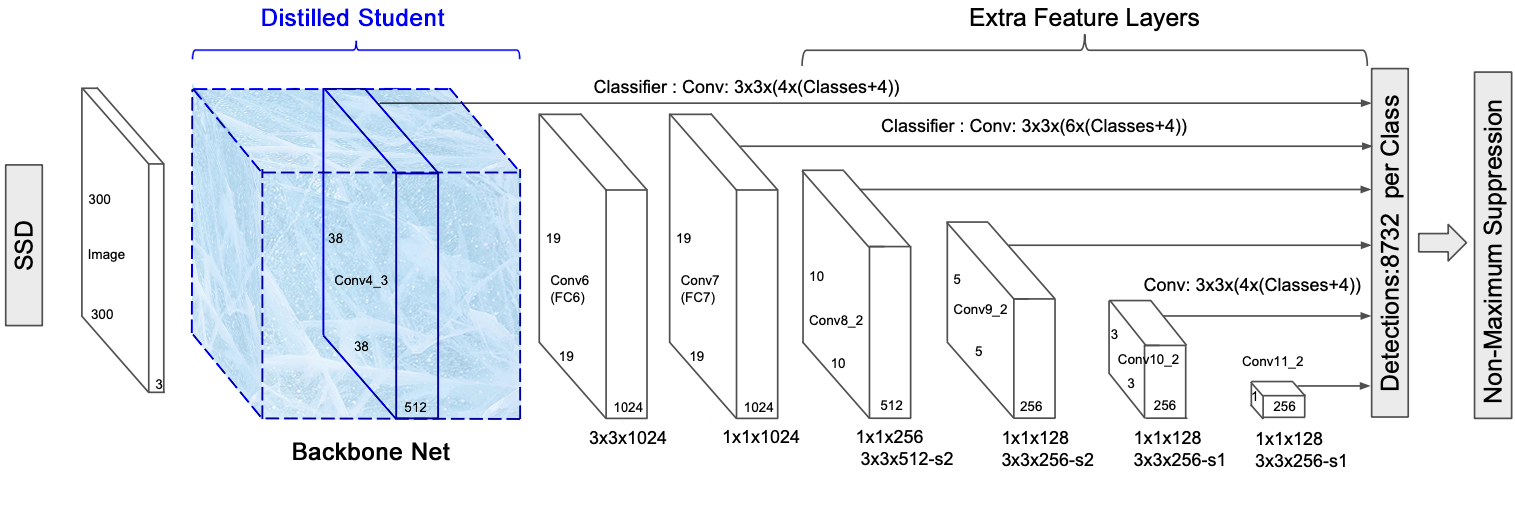
\includegraphics[width = \linewidth]{SSD_architecture_freeze.png}
        \centering
    \end{figure}
    \vspace{-0.5cm}
    \begin{minipage}{\linewidth}
        \centering
        \begin{minipage}{0.40\linewidth}
            {\footnotesize
                \vspace{-0.3cm}
                \begin{block}{\centering 5. Integrazione}
                    Studente distillato come rete "{\bfseries{\emph{backbone}}}" nell'architettura {Single-Shot-Detector (SSD)}.    
                \end{block}
                \vspace{-0.2cm}
                \begin{block}{\centering 6. Freeze}
                    "{\bfseries{\emph{Congelamento}}}"della rete \emph{backbone} durante \emph{l'allenamento} del modello (DSSD).
                \end{block}
            }%
        \end{minipage}
        %\hspace{0.5cm}
        \begin{minipage}{0.55\linewidth}
            \begin{figure}
                \centering
                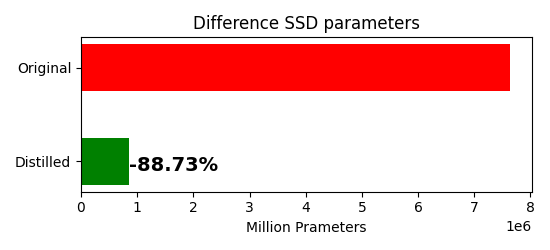
\includegraphics[width = 0.8\linewidth]{Difference SSD parameters.png}
                \centering
            \end{figure}
            \vspace{-0.7cm}
            \begin{figure}
                \centering
                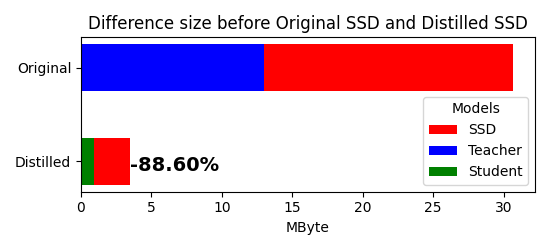
\includegraphics[width = 0.8\linewidth]{Different size SSD.png}
                \centering
            \end{figure}
        \end{minipage}
        \vspace{-2.5cm}
        %{\vspace{-2.5cm}\hspace{-1cm}\reflectbox{\rotatebox[origin=c]{90}{\fontsize{18mm}{19mm}\selectfont{$\curvearrowleft$}}}}
    \end{minipage}   
    \begin{textblock}{10}(109,65)
        \reflectbox{\rotatebox[origin=c]{90}{\fontsize{20mm}{15mm}\selectfont{\transparent{0.2}$\curvearrowleft$}}}
    \end{textblock}
\end{frame}



\begin{frame}{RISULTATI SPERIMENTALI - DSSD (INFERENZA)}
    \renewcommand{\thefootnote}{\fnsymbol{footnote}}
    Differenza \emph{Frames-Per-Second (FPS)} medi tra il modello di partenza 
    {\color{red}{\bfseries{\emph{SSD}}}} e il modello proposto {\color{OliveGreen}{\bfseries{\emph{DSSD}}}}. Benchmark\footnotemark[1] svolti con gli acceleratori 
    \emph{TensorRT} e \emph{OpenCV(cuDNN)} su tutte e tre le architetture di riferimento.\\
    \vspace{0.2cm}
    \begin{minipage}{\linewidth}
        \centering
        \begin{minipage}{0.45\linewidth}
            \begin{figure}
                \centering
                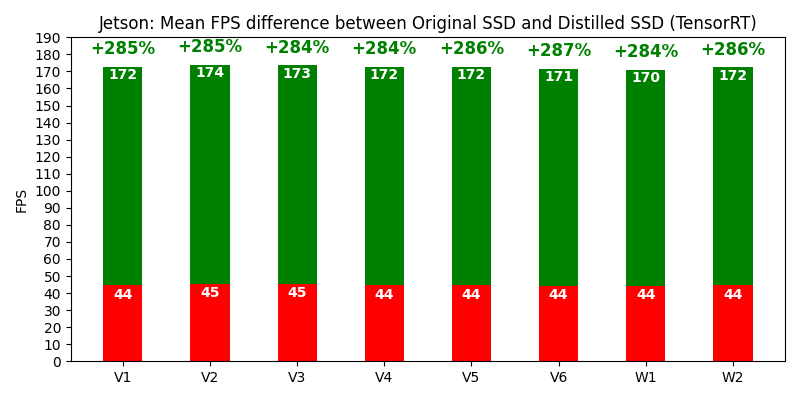
\includegraphics[width = \linewidth]{Mean Difference FPS Jetson TensorRT.png}
                \centering
                \vspace{-0.7cm} 
                \caption{{\bfseries{\emph{Jetson Nano (TensorRT)}}}}
            \end{figure}
        \end{minipage}
        \begin{minipage}{0.45\linewidth}
            \begin{figure}
                \centering
                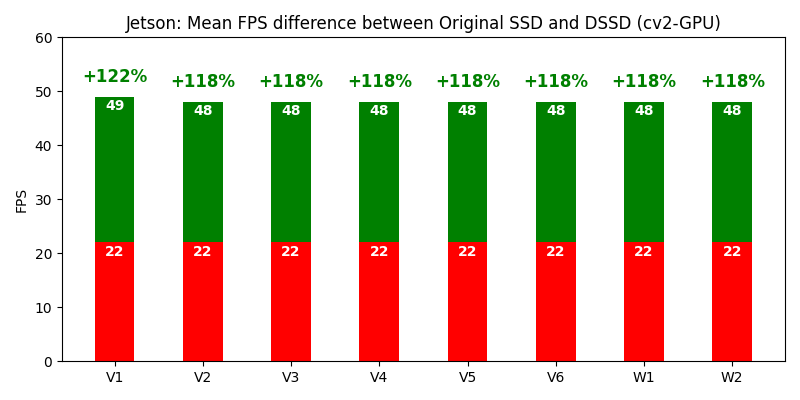
\includegraphics[width = \linewidth]{Difference FPS Jetson cv2 Cuda.png}
                \centering
                \vspace{-0.7cm} 
                \caption{{\bfseries{\emph{Jetson Nano (OpenCV - GPU)}}}}
            \end{figure}
        \end{minipage}
    \end{minipage}
    \begin{minipage}{\linewidth}
        \centering
        \begin{minipage}{0.45\linewidth}
            \begin{figure}
                \centering
                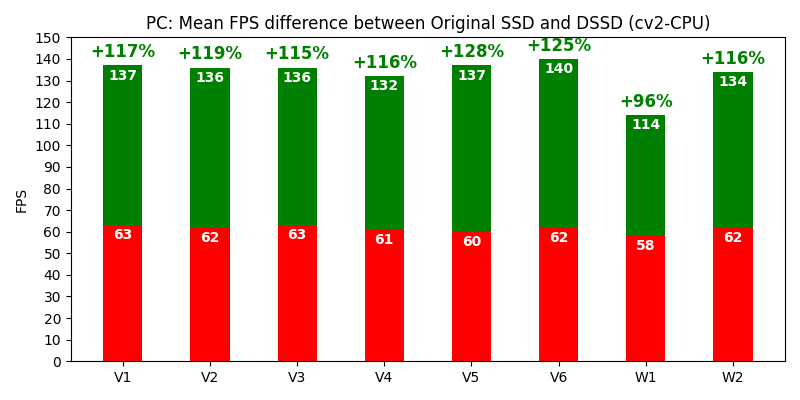
\includegraphics[width = \linewidth]{Mean Difference FPS pc only CPU.png}
                \centering
                \vspace{-0.7cm} 
                \caption{{\bfseries{\emph{Macbook Pro (OpenCV - CPU)}}}}
            \end{figure}
        \end{minipage}
        \begin{minipage}{0.45\linewidth}
            \begin{figure}
                \centering
                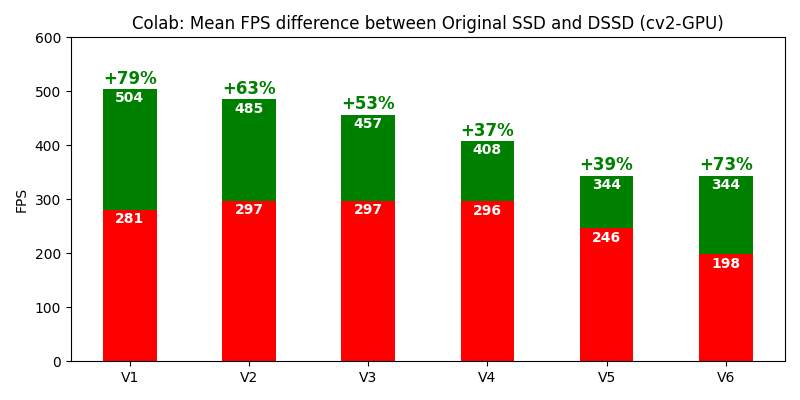
\includegraphics[width = \linewidth]{Mean Difference FPS Colab only GPU.png}
                \centering
                \vspace{-0.7cm} 
                \caption{{\bfseries{\emph{Google Colab (OpenCV - GPU)}}}}
            \end{figure}
        \end{minipage}
    \end{minipage}
    \footnotetext[1]{\scriptsize Sorgenti input: 6 Video (V) e 2 Webcam (W), tutti con differenti risoluzioni.}
\end{frame}

\begin{frame}{ESEMPI OBJECT DETECTION - SSD Vs. DSSD}
    \centering{\color{red}{\bfseries{\Large SSD}}}
    \begin{minipage}{\linewidth}
        \vspace{0.3cm}
        \begin{minipage}{0.32\linewidth}
            \begin{figure}
                \centering
                \vspace{-0.04cm}
                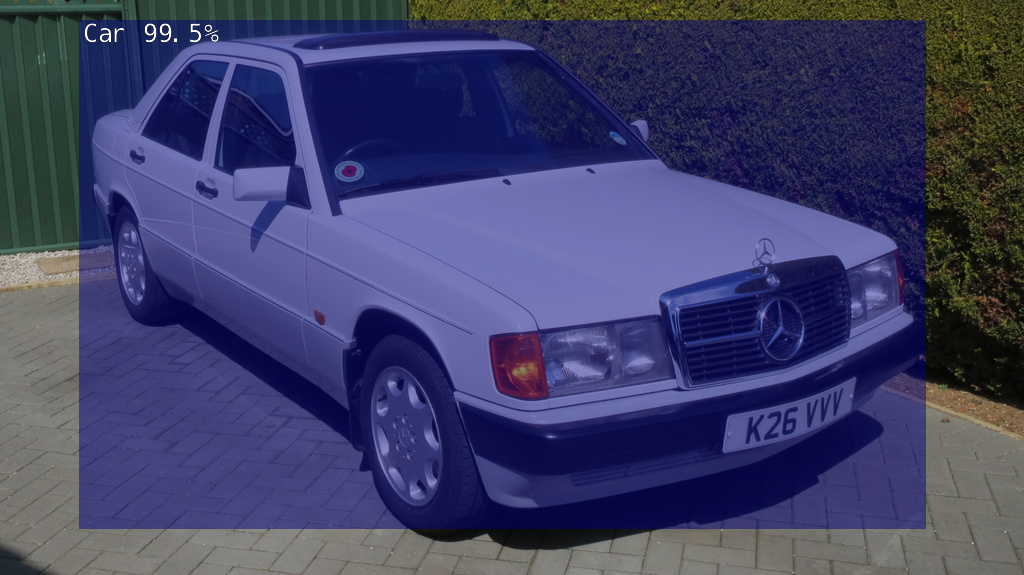
\includegraphics[width=1.2\linewidth]{167_SSD.jpg}
                \caption{99.5\%}
            \end{figure}
        \end{minipage}
        \hspace{0.35cm}
        \begin{minipage}{0.32\linewidth}
            \begin{figure}
                \centering
                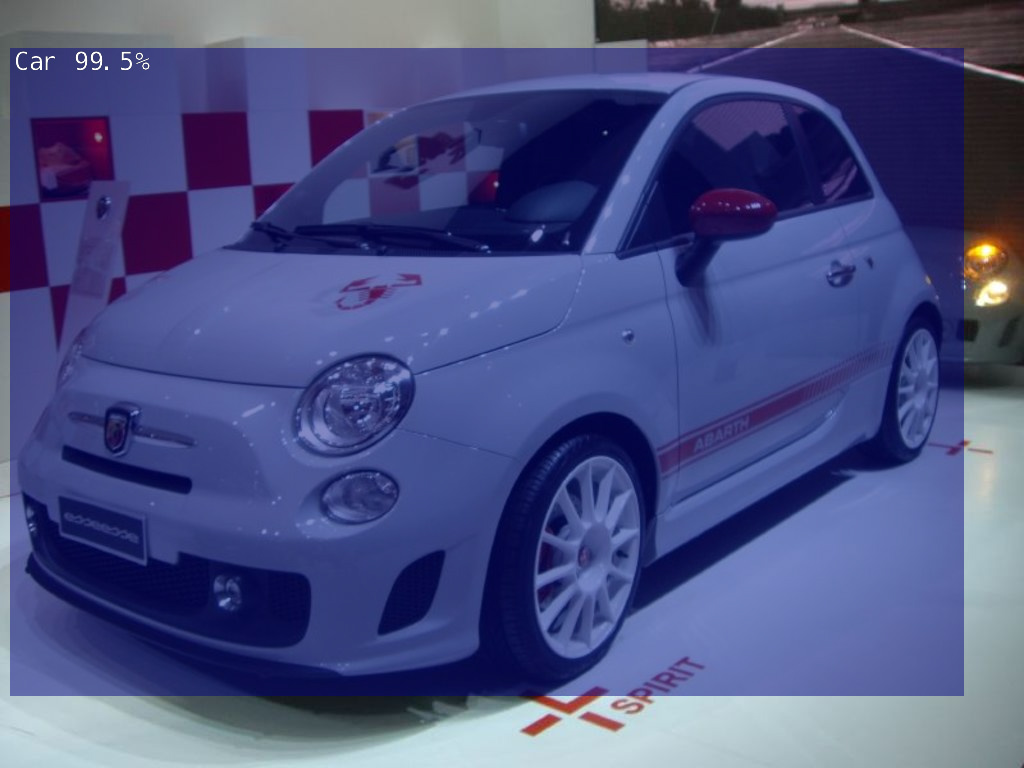
\includegraphics[width=0.8987\linewidth]{131_SSD.jpg}
                \caption{99.5\%}
            \end{figure}
        \end{minipage}
        \hspace{-0.50cm}
        \begin{minipage}{0.32\linewidth}
            \begin{figure}
                \centering
                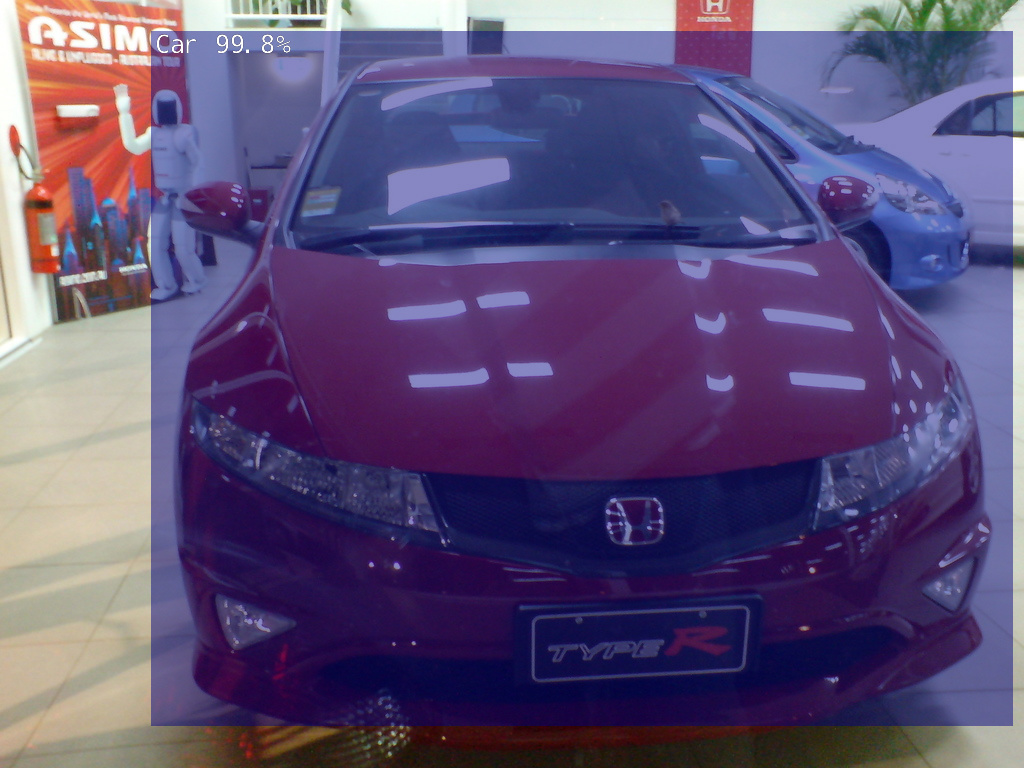
\includegraphics[width=0.899\linewidth]{411_SSD.jpg}  
                \caption{99.8\%}
            \end{figure}
        \end{minipage}
    \end{minipage}  
    \dotfill
    %\vspace{-1cm}
    {\hspace*{-0.3cm}\rule{\textwidth}{1pt}}\\
    \vspace{0.3cm}
    \centering{\bfseries{\color{OliveGreen}{\Large DSSD}}}  
    \begin{minipage}{\linewidth}
        \vspace{0.3cm}
        \begin{minipage}{0.32\linewidth}
            \begin{figure}
                \centering
                \vspace{-0.04cm}
                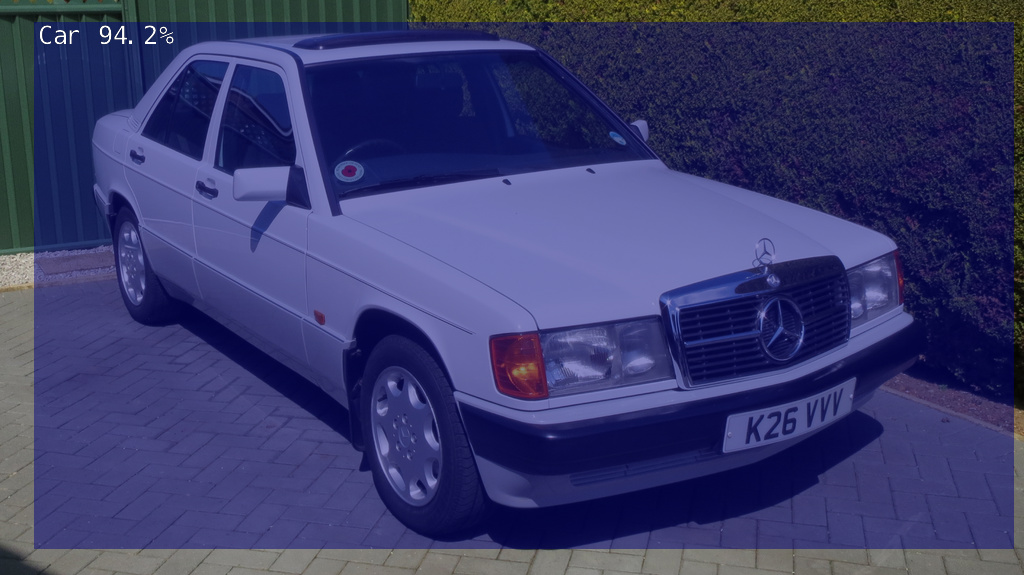
\includegraphics[width=1.2\linewidth]{167_DSSD.jpg}
                \caption{94.2\%}
            \end{figure}
        \end{minipage}
        \hspace{0.35cm}
        \begin{minipage}{0.32\linewidth}
            \begin{figure}
                \centering
                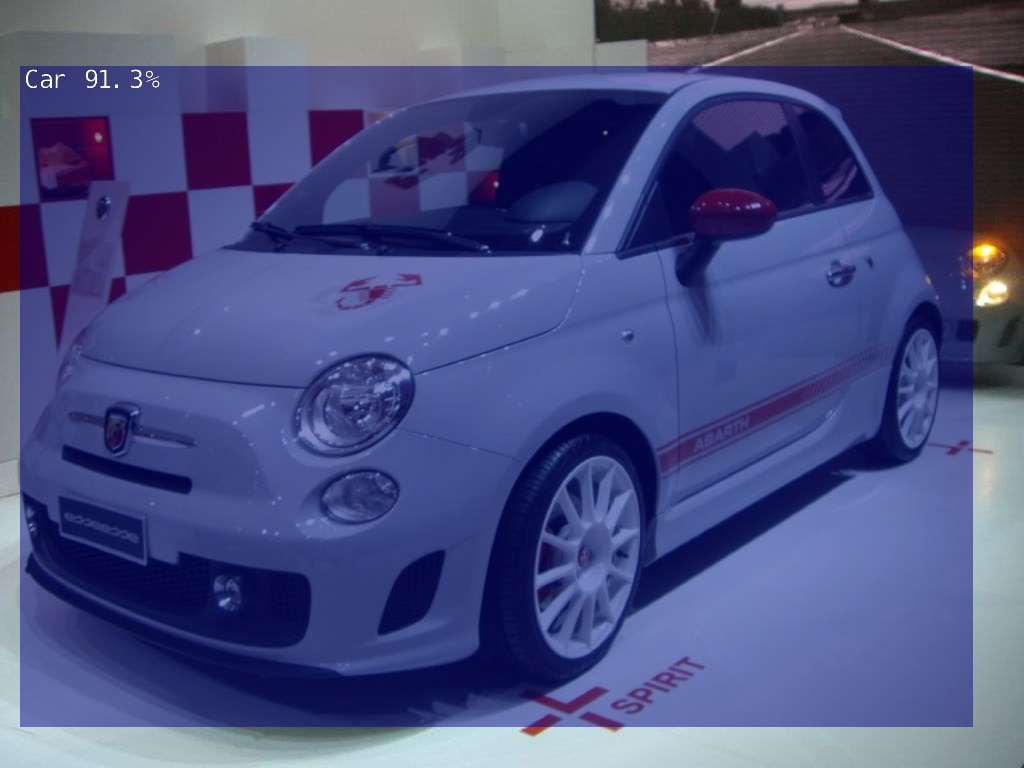
\includegraphics[width=0.8987\linewidth]{131_DSSD.jpg}
                \caption{91.3\%}
            \end{figure}
        \end{minipage}
        \hspace{-0.50cm}
        \begin{minipage}{0.32\linewidth}
            \begin{figure}
                \centering
                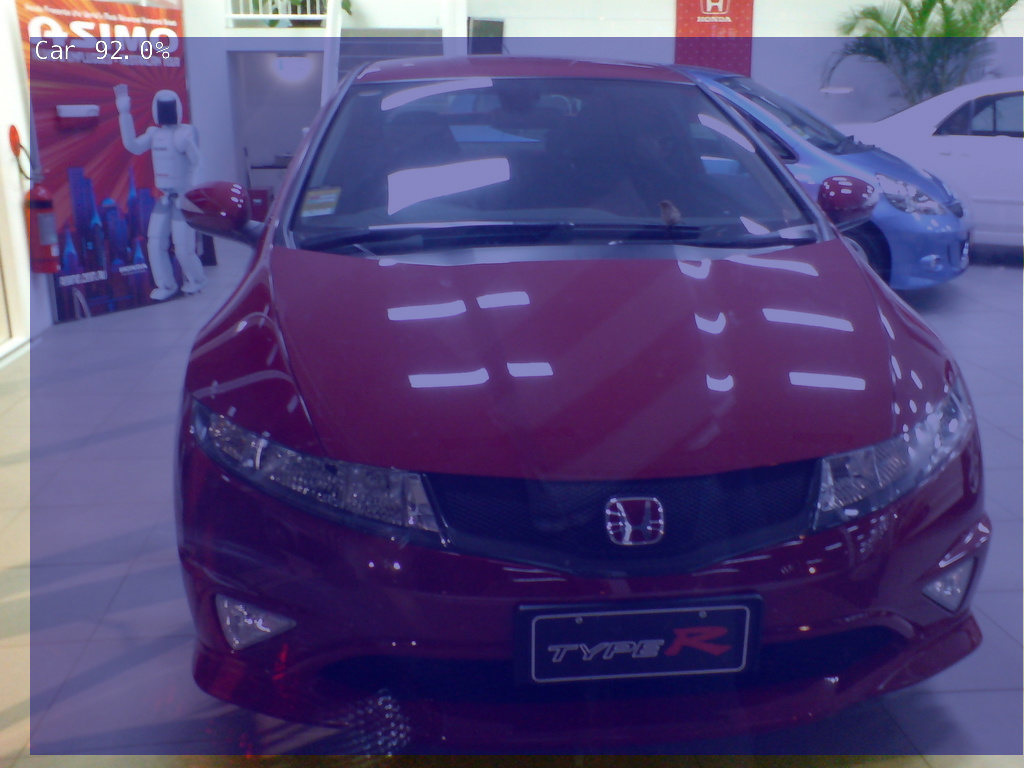
\includegraphics[width=0.899\linewidth]{411_DSSD.jpg}  
                \caption{92\%}
            \end{figure}
        \end{minipage}
    \end{minipage}   
\end{frame}



\end{document}